\documentclass[12pt]{article}
\newcommand{\gradeband}{Grades 2–3}
% Shared layout for the Week 7 student pages (compile with xelatex)
\usepackage[letterpaper, top=0.95in, bottom=0.75in, left=0.8in, right=0.8in,
            headheight=20pt, headsep=16pt, footskip=28pt]{geometry}
\usepackage{fontspec}
\setmainfont{Andika}
\usepackage{xcolor}
\usepackage{tikz}
\usetikzlibrary{arrows.meta,positioning,calc}
\usepackage[most]{tcolorbox}
\usepackage{fancyhdr}

\pagestyle{fancy}
\fancyhf{}
\lhead{\small Bellingham Math Circle \enspace\textperiodcentered\enspace Week 7
       \enspace\textperiodcentered\enspace \gradeband}
\rhead{\small Name \rule[-2pt]{5cm}{0.5pt}}
\cfoot{\small \thepage}
\renewcommand{\headrulewidth}{0.4pt}

\setlength{\parindent}{0pt}
\setlength{\parskip}{5pt}
\hyphenpenalty=10000
\exhyphenpenalty=10000
\AtBeginDocument{\raggedright}

\newcounter{prob}
\newcommand{\problem}{\stepcounter{prob}\par\textbf{Problem \theprob:}\enspace}

\newtcolorbox{rulebox}{enhanced, colback=white, colframe=black!55,
  boxrule=0.7pt, arc=2mm, left=8pt, right=8pt, top=6pt, bottom=6pt,
  before upper=\raggedright}

% ---- counters -------------------------------------------------------------
\tikzset{
  ctr/.style={circle, draw=black, fill=black!18, line width=0.6pt,
              minimum size=#1, inner sep=0pt},
  ctr/.default=5mm,
  xmark/.style={line width=1.4pt, line cap=round},
  ansbox/.style={draw=black, line width=0.6pt, minimum size=#1, inner sep=0pt},
  ansbox/.default=9mm,
}
% \pile[size]{n}{crossed}{per row}{step}  (drawn with top-left counter at origin)
\newcommand{\pile}[5][5mm]{%
  \foreach \i in {1,...,#2} {%
    \pgfmathtruncatemacro{\col}{mod(\i-1,#4)}%
    \pgfmathtruncatemacro{\row}{(\i-1)/#4}%
    \node[ctr=#1] (p\i) at (\col*#5, -\row*#5) {};%
    \pgfmathtruncatemacro{\thr}{#2-#3}%
    \ifnum\i>\thr
      \draw[xmark] ($(p\i)+(-0.62*#1,0.62*#1)$) -- ($(p\i)+(0.62*#1,-0.62*#1)$)
                   ($(p\i)+(0.62*#1,0.62*#1)$) -- ($(p\i)+(-0.62*#1,-0.62*#1)$);
    \fi
  }}

\usepackage{array}

% W/L table: \wltable{first}{last} in rows of 10
\newcommand{\wltable}[2]{%
  \begin{tikzpicture}[x=1.62cm, y=1cm]
    \foreach \n in {#1,...,#2} {
      \pgfmathtruncatemacro{\k}{\n-#1}
      \pgfmathsetmacro{\cx}{mod(\k,10)}
      \pgfmathsetmacro{\cy}{-2.45*int(\k/10)}
      \fill[black!10] (\cx,\cy) rectangle ++(1,-0.8);
      \draw[line width=0.6pt] (\cx,\cy) rectangle ++(1,-0.8);
      \draw[line width=0.6pt] (\cx,\cy-0.8) rectangle ++(1,-1.2);
      \node[font=\bfseries, text height=1.6ex, text depth=0.2ex] at (\cx+0.5,\cy-0.4) {\n};
    }
  \end{tikzpicture}}

% two piles in outlines, up to 10 counters each
\newcommand{\twopiles}[2]{%
  \begin{tikzpicture}[baseline={(0,0.8)}]
    \draw[rounded corners=3mm, line width=0.6pt, black!60] (0,0) rectangle (3.8,1.7);
    \begin{scope}[shift={(0.5,1.2)}]\pile[5mm]{#1}{0}{5}{0.7}\end{scope}
    \draw[rounded corners=3mm, line width=0.6pt, black!60] (4.3,0) rectangle (8.1,1.7);
    \begin{scope}[shift={(4.8,1.2)}]\pile[5mm]{#2}{0}{5}{0.7}\end{scope}
    \node[font=\small] at (1.9,-0.3) {#1};
    \node[font=\small] at (6.2,-0.3) {#2};
  \end{tikzpicture}}

\newcommand{\choice}[1]{\tikz[baseline=(t.base)]\node[draw, rounded corners=2mm,
  line width=0.6pt, inner xsep=8pt, inner ysep=5pt] (t) {#1};}

\begin{document}
\fontsize{13}{18.5}\selectfont
\setlength{\parskip}{6pt}

\begin{rulebox}
Two players share one pile of counters and take turns. On each turn a player
takes away 1, 3, or 4 counters, and nobody may take more counters than the pile
has. Whoever takes the last counter wins.

\smallskip
A pile is a \textbf{losing pile} if the player whose turn it is will lose when
the other player plays carefully. A pile is a \textbf{winning pile} if the
player whose turn it is can win, whatever the other player does.
\end{rulebox}

\medskip
\problem Play the game several times with a pile of 6 counters, taking turns
going first. Which player can always win from 6, the first player or the
second player? Write how that player wins.

\vspace{6.2cm}

\problem Write W under each winning pile and L under each losing pile.

\medskip
\begin{center}
\wltable{1}{20}
\end{center}

\vfill
\newpage

\problem A player claims: “If the pile has at least 4 counters and you can
win, then taking 4 counters is a way to win.” Is the claim correct?

\vspace{8.5cm}

\problem A player claims: “With a pile of 8 counters, the second
player can always win by taking the same number of counters the first player
just took.” Is the claim correct?

\vfill
\newpage

\problem This table shows a game that started with 16 counters. Find every
turn where the player could have taken a different number of counters and
then been sure to win.

\medskip
\begin{center}
\renewcommand{\arraystretch}{1.55}
\begin{tabular}{|>{\centering\arraybackslash}p{1.6cm}|>{\centering\arraybackslash}p{3.4cm}
                |>{\centering\arraybackslash}p{2.6cm}|>{\centering\arraybackslash}p{2.6cm}
                |>{\centering\arraybackslash}p{2.6cm}|}
\hline
\textbf{turn} & \textbf{player} & \textbf{pile before} & \textbf{taken} & \textbf{pile after} \\
\hline
1 & first  & 16 & 1 & 15 \\ \hline
2 & second & 15 & 4 & 11 \\ \hline
3 & first  & 11 & 1 & 10 \\ \hline
4 & second & 10 & 3 & 7  \\ \hline
5 & first  & 7  & 4 & 3  \\ \hline
6 & second & 3  & 3 & 0  \\ \hline
\end{tabular}
\end{center}

\vspace{4.6cm}

\problem With a pile of 14 counters, which player can always win? Write a plan
for that player that works against every move the other player might make.

\vfill
\newpage

\problem For each pile, write W in its box if it is a winning pile and L if it
is a losing pile. Write how you know the answer for 100.

\medskip
\begin{center}
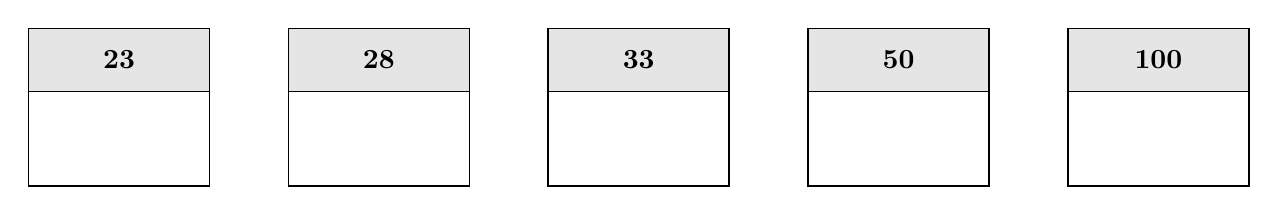
\begin{tikzpicture}[x=1cm,y=1cm]
  \foreach \n [count=\i] in {23, 28, 33, 50, 100} {
    \pgfmathsetmacro{\cx}{(\i-1)*3.3}
    \fill[black!10] (\cx,0) rectangle ++(2.3,-0.8);
    \draw[line width=0.6pt] (\cx,0) rectangle ++(2.3,-0.8);
    \draw[line width=0.6pt] (\cx,-0.8) rectangle ++(2.3,-1.2);
    \node[font=\bfseries, text height=1.6ex, text depth=0.2ex] at (\cx+1.15,-0.4) {\n};
  }
\end{tikzpicture}
\end{center}

\vspace{4.8cm}

\problem Play with a different rule: on each turn a player takes away 1, 3, or
5 counters. Whoever takes the last counter wins. Write W under each winning
pile and L under each losing pile. Then describe all the losing piles,
including piles larger than 20.

\medskip
\begin{center}
\wltable{1}{20}
\end{center}

\vfill
\newpage

\problem Now there are two piles. On each turn a player chooses one pile and
takes 1, 3, or 4 counters from that pile only. Whoever takes the last counter
wins. For each start, circle the player who can always win.

\medskip
\begin{center}
\renewcommand{\arraystretch}{1}
\begin{tabular}{@{}l@{\hspace{1cm}}c@{\hspace{0.5cm}}c@{}}
\twopiles{5}{5} & \choice{first player} & \choice{second player} \\[2.2cm]
\twopiles{7}{2} & \choice{first player} & \choice{second player} \\[2.2cm]
\twopiles{6}{1} & \choice{first player} & \choice{second player} \\[2.2cm]
\twopiles{9}{8} & \choice{first player} & \choice{second player} \\[2.2cm]
\twopiles{6}{4} & \choice{first player} & \choice{second player} \\
\end{tabular}
\end{center}

\vfill
\end{document}
